\documentclass[1p]{elsarticle_modified}
%\bibliographystyle{elsarticle-num}

%\usepackage[colorlinks]{hyperref}
%\usepackage{abbrmath_seonhwa} %\Abb, \Ascr, \Acal ,\Abf, \Afrak
\usepackage{amsfonts}
\usepackage{amssymb}
\usepackage{amsmath}
\usepackage{amsthm}
\usepackage{scalefnt}
\usepackage{amsbsy}
\usepackage{kotex}
\usepackage{caption}
\usepackage{subfig}
\usepackage{color}
\usepackage{graphicx}
\usepackage{xcolor} %% white, black, red, green, blue, cyan, magenta, yellow
\usepackage{float}
\usepackage{setspace}
\usepackage{hyperref}

\usepackage{tikz}
\usetikzlibrary{arrows}

\usepackage{multirow}
\usepackage{array} % fixed length table
\usepackage{hhline}

%%%%%%%%%%%%%%%%%%%%%
\makeatletter
\renewcommand*\env@matrix[1][\arraystretch]{%
	\edef\arraystretch{#1}%
	\hskip -\arraycolsep
	\let\@ifnextchar\new@ifnextchar
	\array{*\c@MaxMatrixCols c}}
\makeatother %https://tex.stackexchange.com/questions/14071/how-can-i-increase-the-line-spacing-in-a-matrix
%%%%%%%%%%%%%%%

\usepackage[normalem]{ulem}

\newcommand{\msout}[1]{\ifmmode\text{\sout{\ensuremath{#1}}}\else\sout{#1}\fi}
%SOURCE: \msout is \stkout macro in https://tex.stackexchange.com/questions/20609/strikeout-in-math-mode

\newcommand{\cancel}[1]{
	\ifmmode
	{\color{red}\msout{#1}}
	\else
	{\color{red}\sout{#1}}
	\fi
}

\newcommand{\add}[1]{
	{\color{blue}\uwave{#1}}
}

\newcommand{\replace}[2]{
	\ifmmode
	{\color{red}\msout{#1}}{\color{blue}\uwave{#2}}
	\else
	{\color{red}\sout{#1}}{\color{blue}\uwave{#2}}
	\fi
}

\newcommand{\Sol}{\mathcal{S}} %segment
\newcommand{\D}{D} %diagram
\newcommand{\A}{\mathcal{A}} %arc


%%%%%%%%%%%%%%%%%%%%%%%%%%%%%5 test

\def\sl{\operatorname{\textup{SL}}(2,\Cbb)}
\def\psl{\operatorname{\textup{PSL}}(2,\Cbb)}
\def\quan{\mkern 1mu \triangleright \mkern 1mu}

\theoremstyle{definition}
\newtheorem{thm}{Theorem}[section]
\newtheorem{prop}[thm]{Proposition}
\newtheorem{lem}[thm]{Lemma}
\newtheorem{ques}[thm]{Question}
\newtheorem{cor}[thm]{Corollary}
\newtheorem{defn}[thm]{Definition}
\newtheorem{exam}[thm]{Example}
\newtheorem{rmk}[thm]{Remark}
\newtheorem{alg}[thm]{Algorithm}

\newcommand{\I}{\sqrt{-1}}
\begin{document}

%\begin{frontmatter}
%
%\title{Boundary parabolic representations of knots up to 8 crossings}
%
%%% Group authors per affiliation:
%\author{Yunhi Cho} 
%\address{Department of Mathematics, University of Seoul, Seoul, Korea}
%\ead{yhcho@uos.ac.kr}
%
%
%\author{Seonhwa Kim} %\fnref{s_kim}}
%\address{Center for Geometry and Physics, Institute for Basic Science, Pohang, 37673, Korea}
%\ead{ryeona17@ibs.re.kr}
%
%\author{Hyuk Kim}
%\address{Department of Mathematical Sciences, Seoul National University, Seoul 08826, Korea}
%\ead{hyukkim@snu.ac.kr}
%
%\author{Seokbeom Yoon}
%\address{Department of Mathematical Sciences, Seoul National University, Seoul, 08826,  Korea}
%\ead{sbyoon15@snu.ac.kr}
%
%\begin{abstract}
%We find all boundary parabolic representation of knots up to 8 crossings.
%
%\end{abstract}
%\begin{keyword}
%    \MSC[2010] 57M25 
%\end{keyword}
%
%\end{frontmatter}

%\linenumbers
%\tableofcontents
%
\newcommand\colored[1]{\textcolor{white}{\rule[-0.35ex]{0.8em}{1.4ex}}\kern-0.8em\color{red} #1}%
%\newcommand\colored[1]{\textcolor{white}{ #1}\kern-2.17ex	\textcolor{white}{ #1}\kern-1.81ex	\textcolor{white}{ #1}\kern-2.15ex\color{red}#1	}

{\Large $\underline{12n_{0630}~(K12n_{0630})}$}

\setlength{\tabcolsep}{10pt}
\renewcommand{\arraystretch}{1.6}
\vspace{1cm}\begin{tabular}{m{100pt}>{\centering\arraybackslash}m{274pt}}
\multirow{5}{120pt}{
	\centering
	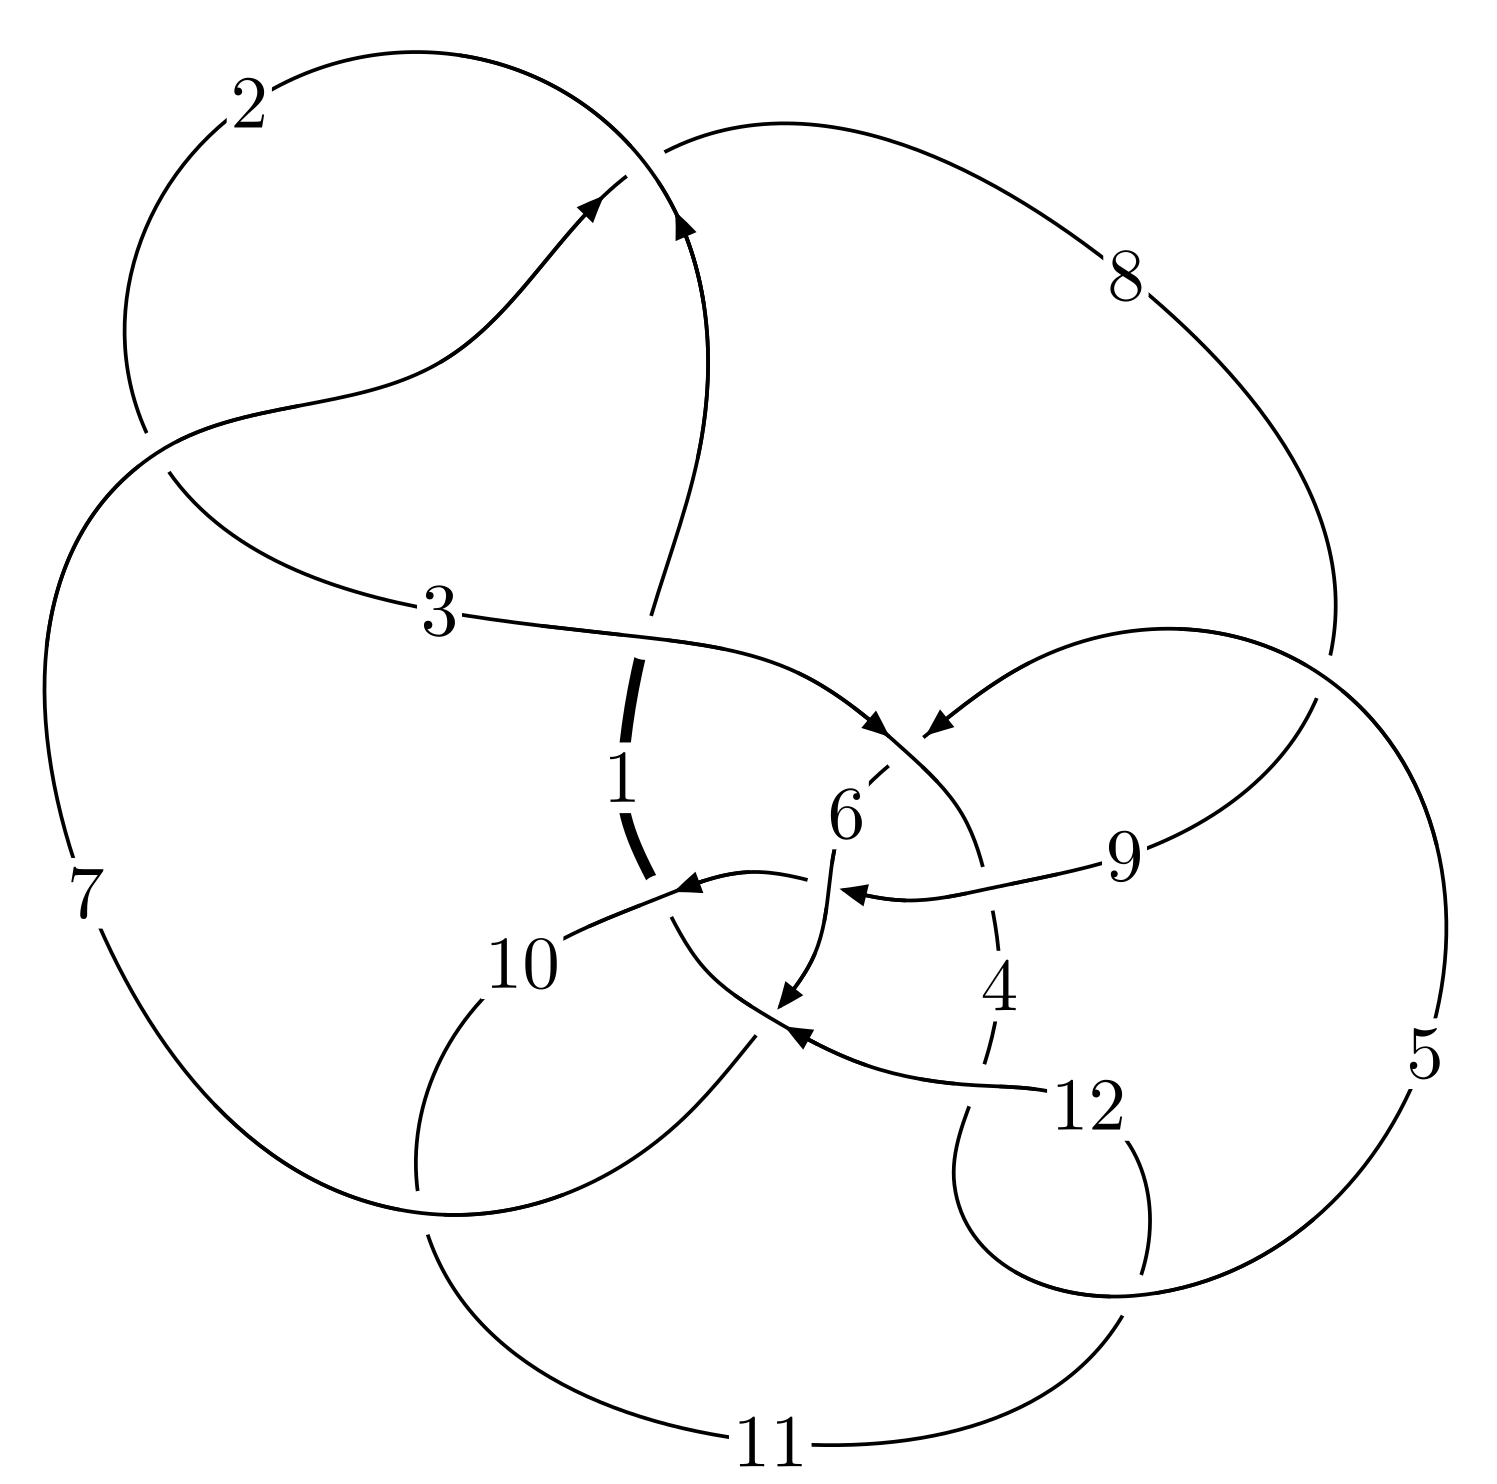
\includegraphics[width=112pt]{../../../GIT/diagram.site/Diagrams/png/2719_12n_0630.png}\\
\ \ \ A knot diagram\footnotemark}&
\allowdisplaybreaks
\textbf{Linearized knot diagam} \\
\cline{2-2}
 &
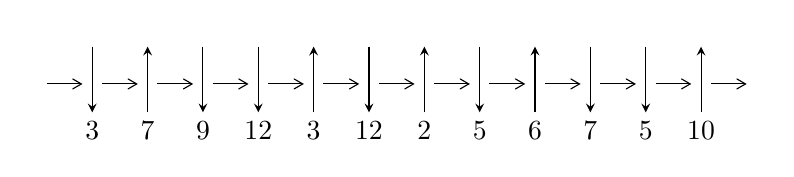
\begin{tikzpicture}[x=20pt, y=17pt]
	% nodes
	\node (C0) at (0, 0) {};
	\node (C1) at (1, 0) {};
	\node (C1U) at (1, +1) {};
	\node (C1D) at (1, -1) {3};

	\node (C2) at (2, 0) {};
	\node (C2U) at (2, +1) {};
	\node (C2D) at (2, -1) {7};

	\node (C3) at (3, 0) {};
	\node (C3U) at (3, +1) {};
	\node (C3D) at (3, -1) {9};

	\node (C4) at (4, 0) {};
	\node (C4U) at (4, +1) {};
	\node (C4D) at (4, -1) {12};

	\node (C5) at (5, 0) {};
	\node (C5U) at (5, +1) {};
	\node (C5D) at (5, -1) {3};

	\node (C6) at (6, 0) {};
	\node (C6U) at (6, +1) {};
	\node (C6D) at (6, -1) {12};

	\node (C7) at (7, 0) {};
	\node (C7U) at (7, +1) {};
	\node (C7D) at (7, -1) {2};

	\node (C8) at (8, 0) {};
	\node (C8U) at (8, +1) {};
	\node (C8D) at (8, -1) {5};

	\node (C9) at (9, 0) {};
	\node (C9U) at (9, +1) {};
	\node (C9D) at (9, -1) {6};

	\node (C10) at (10, 0) {};
	\node (C10U) at (10, +1) {};
	\node (C10D) at (10, -1) {7};

	\node (C11) at (11, 0) {};
	\node (C11U) at (11, +1) {};
	\node (C11D) at (11, -1) {5};

	\node (C12) at (12, 0) {};
	\node (C12U) at (12, +1) {};
	\node (C12D) at (12, -1) {10};
	\node (C13) at (13, 0) {};

	% arrows
	\draw[->,>={angle 60}]
	(C0) edge (C1) (C1) edge (C2) (C2) edge (C3) (C3) edge (C4) (C4) edge (C5) (C5) edge (C6) (C6) edge (C7) (C7) edge (C8) (C8) edge (C9) (C9) edge (C10) (C10) edge (C11) (C11) edge (C12) (C12) edge (C13) ;	\draw[->,>=stealth]
	(C1U) edge (C1D) (C2D) edge (C2U) (C3U) edge (C3D) (C4U) edge (C4D) (C5D) edge (C5U) (C6U) edge (C6D) (C7D) edge (C7U) (C8U) edge (C8D) (C9D) edge (C9U) (C10U) edge (C10D) (C11U) edge (C11D) (C12D) edge (C12U) ;
	\end{tikzpicture} \\
\hhline{~~} \\& 
\textbf{Solving Sequence} \\ \cline{2-2} 
 &
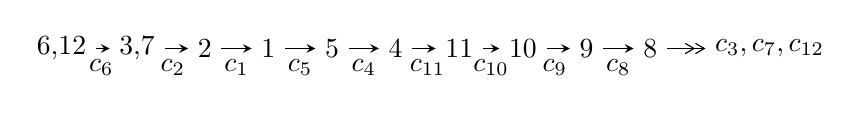
\begin{tikzpicture}[x=23pt, y=7pt]
	% node
	\node (A0) at (-1/8, 0) {6,12};
	\node (A1) at (17/16, 0) {3,7};
	\node (A2) at (17/8, 0) {2};
	\node (A3) at (25/8, 0) {1};
	\node (A4) at (33/8, 0) {5};
	\node (A5) at (41/8, 0) {4};
	\node (A6) at (49/8, 0) {11};
	\node (A7) at (57/8, 0) {10};
	\node (A8) at (65/8, 0) {9};
	\node (A9) at (73/8, 0) {8};
	\node (C1) at (1/2, -1) {$c_{6}$};
	\node (C2) at (13/8, -1) {$c_{2}$};
	\node (C3) at (21/8, -1) {$c_{1}$};
	\node (C4) at (29/8, -1) {$c_{5}$};
	\node (C5) at (37/8, -1) {$c_{4}$};
	\node (C6) at (45/8, -1) {$c_{11}$};
	\node (C7) at (53/8, -1) {$c_{10}$};
	\node (C8) at (61/8, -1) {$c_{9}$};
	\node (C9) at (69/8, -1) {$c_{8}$};
	\node (A10) at (11, 0) {$c_{3},c_{7},c_{12}$};

	% edge
	\draw[->,>=stealth]	
	(A0) edge (A1) (A1) edge (A2) (A2) edge (A3) (A3) edge (A4) (A4) edge (A5) (A5) edge (A6) (A6) edge (A7) (A7) edge (A8) (A8) edge (A9) ;
	\draw[->>,>={angle 60}]	
	(A9) edge (A10);
\end{tikzpicture} \\ 

\end{tabular} \\

\footnotetext{
The image of knot diagram is generated by the software ``\textbf{Draw programme}" developed by Andrew Bartholomew(\url{http://www.layer8.co.uk/maths/draw/index.htm\#Running-draw}), where we modified some parts for our purpose(\url{https://github.com/CATsTAILs/LinksPainter}).
}\phantom \\ \newline 
\centering \textbf{Ideals for irreducible components\footnotemark of $X_{\text{par}}$} 
 
\begin{align*}
I^u_{1}&=\langle 
-397668 u^{11}-278148 u^{10}+\cdots+7297577 b+2368848,\\
\phantom{I^u_{1}}&\phantom{= \langle  }-1957869 u^{11}+467354 u^{10}+\cdots+36487885 a-28305373,\\
\phantom{I^u_{1}}&\phantom{= \langle  }u^{12}- u^{11}-6 u^{10}+13 u^9+18 u^8-60 u^7+13 u^6+62 u^5-29 u^4-23 u^3+7 u^2+2 u+5\rangle \\
I^u_{2}&=\langle 
-3.02231\times10^{15} u^{19}+1.19819\times10^{15} u^{18}+\cdots+5.91941\times10^{15} b+5.59657\times10^{14},\\
\phantom{I^u_{2}}&\phantom{= \langle  }9227751817881066 u^{19}+3660231888309292 u^{18}+\cdots+5919405752257771 a+5607818622219472,\\
\phantom{I^u_{2}}&\phantom{= \langle  }u^{20}+4 u^{18}+\cdots+3 u+1\rangle \\
I^u_{3}&=\langle 
-2.64152\times10^{16} u^{15}-7.92608\times10^{15} u^{14}+\cdots+8.40192\times10^{18} b+2.48982\times10^{18},\\
\phantom{I^u_{3}}&\phantom{= \langle  }-2.01301\times10^{18} u^{15}+1.13113\times10^{19} u^{14}+\cdots+5.96536\times10^{20} a+4.26142\times10^{21},\\
\phantom{I^u_{3}}&\phantom{= \langle  }u^{16}- u^{15}+\cdots+163 u+71\rangle \\
I^u_{4}&=\langle 
u^2+b-1,\;u^2+a+u,\;u^3- u+1\rangle \\
I^u_{5}&=\langle 
b- u-1,\;a- u,\;u^2+u+1\rangle \\
\\
\end{align*}
\raggedright * 5 irreducible components of $\dim_{\mathbb{C}}=0$, with total 53 representations.\\
\footnotetext{All coefficients of polynomials are rational numbers. But the coefficients are sometimes approximated in decimal forms when there is not enough margin.}
\newpage
\renewcommand{\arraystretch}{1}
\centering \section*{I. $I^u_{1}= \langle -3.98\times10^{5} u^{11}-2.78\times10^{5} u^{10}+\cdots+7.30\times10^{6} b+2.37\times10^{6},\;-1.96\times10^{6} u^{11}+4.67\times10^{5} u^{10}+\cdots+3.65\times10^{7} a-2.83\times10^{7},\;u^{12}- u^{11}+\cdots+2 u+5 \rangle$}
\flushleft \textbf{(i) Arc colorings}\\
\begin{tabular}{m{7pt} m{180pt} m{7pt} m{180pt} }
\flushright $a_{6}=$&$\begin{pmatrix}1\\0\end{pmatrix}$ \\
\flushright $a_{12}=$&$\begin{pmatrix}0\\u\end{pmatrix}$ \\
\flushright $a_{3}=$&$\begin{pmatrix}0.0536581 u^{11}-0.0128085 u^{10}+\cdots+0.801672 u+0.775747\\0.0544932 u^{11}+0.0381151 u^{10}+\cdots+0.115543 u-0.324607\end{pmatrix}$ \\
\flushright $a_{7}=$&$\begin{pmatrix}1\\u^2\end{pmatrix}$ \\
\flushright $a_{2}=$&$\begin{pmatrix}0.109535 u^{11}-0.0184761 u^{10}+\cdots+0.336139 u+0.896107\\0.268311 u^{11}+0.00905821 u^{10}+\cdots-0.264263 u-0.575656\end{pmatrix}$ \\
\flushright $a_{1}=$&$\begin{pmatrix}0.0908787 u^{11}+0.0231775 u^{10}+\cdots+0.150881 u+0.429910\\0.255543 u^{11}-0.178786 u^{10}+\cdots-0.0241484 u+0.207817\end{pmatrix}$ \\
\flushright $a_{5}=$&$\begin{pmatrix}-0.0776514 u^{11}-0.0522672 u^{10}+\cdots+1.20161 u+1.87973\\0.114056 u^{11}+0.0999037 u^{10}+\cdots+0.248152 u-0.454394\end{pmatrix}$ \\
\flushright $a_{4}=$&$\begin{pmatrix}-0.0776514 u^{11}-0.0522672 u^{10}+\cdots+1.20161 u+1.87973\\0.131309 u^{11}+0.0394587 u^{10}+\cdots-0.399942 u-1.10399\end{pmatrix}$ \\
\flushright $a_{11}=$&$\begin{pmatrix}-0.313406 u^{11}+0.172062 u^{10}+\cdots+2.31775 u+0.230813\\0.0700486 u^{11}+0.0126635 u^{10}+\cdots+0.664609 u+0.230518\end{pmatrix}$ \\
\flushright $a_{10}=$&$\begin{pmatrix}-0.0649215 u^{11}+0.0104283 u^{10}+\cdots+1.13264 u-0.245386\\0.155876 u^{11}-0.0790595 u^{10}+\cdots-0.751512 u-0.203733\end{pmatrix}$ \\
\flushright $a_{9}=$&$\begin{pmatrix}-0.220797 u^{11}+0.0894879 u^{10}+\cdots+1.88416 u-0.0416525\\0.155876 u^{11}-0.0790595 u^{10}+\cdots-0.751512 u-0.203733\end{pmatrix}$ \\
\flushright $a_{8}=$&$\begin{pmatrix}0.131232 u^{11}-0.216101 u^{10}+\cdots+0.285872 u+0.275328\\0.0893665 u^{11}+0.00788878 u^{10}+\cdots-0.146247 u-0.586750\end{pmatrix}$\\&\end{tabular}
\flushleft \textbf{(ii) Obstruction class $= -1$}\\~\\
\flushleft \textbf{(iii) Cusp Shapes $= -\frac{5487178}{7297577} u^{11}+\frac{4986967}{7297577} u^{10}+\cdots-\frac{3943475}{384083} u-\frac{53169632}{7297577}$}\\~\\
\newpage\renewcommand{\arraystretch}{1}
\flushleft \textbf{(iv) u-Polynomials at the component}\newline \\
\begin{tabular}{m{50pt}|m{274pt}}
Crossings & \hspace{64pt}u-Polynomials at each crossing \\
\hline $$\begin{aligned}c_{1}\end{aligned}$$&$\begin{aligned}
&u^{12}+22 u^{11}+\cdots+2624 u+256
\end{aligned}$\\
\hline $$\begin{aligned}c_{2},c_{7}\end{aligned}$$&$\begin{aligned}
&u^{12}-4 u^{11}+\cdots-24 u+16
\end{aligned}$\\
\hline $$\begin{aligned}c_{3},c_{6}\end{aligned}$$&$\begin{aligned}
&u^{12}- u^{11}+\cdots+2 u+5
\end{aligned}$\\
\hline $$\begin{aligned}c_{4},c_{11}\end{aligned}$$&$\begin{aligned}
&u^{12}-15 u^{10}+\cdots+425 u+152
\end{aligned}$\\
\hline $$\begin{aligned}c_{5},c_{12}\end{aligned}$$&$\begin{aligned}
&u^{12}+2 u^{11}+\cdots-9 u+7
\end{aligned}$\\
\hline $$\begin{aligned}c_{8},c_{10}\end{aligned}$$&$\begin{aligned}
&u^{12}- u^{11}+\cdots+1494 u+607
\end{aligned}$\\
\hline $$\begin{aligned}c_{9}\end{aligned}$$&$\begin{aligned}
&u^{12}-5 u^{11}+\cdots+31 u+14
\end{aligned}$\\
\hline
\end{tabular}\\~\\
\newpage\renewcommand{\arraystretch}{1}
\flushleft \textbf{(v) Riley Polynomials at the component}\newline \\
\begin{tabular}{m{50pt}|m{274pt}}
Crossings & \hspace{64pt}Riley Polynomials at each crossing \\
\hline $$\begin{aligned}c_{1}\end{aligned}$$&$\begin{aligned}
&y^{12}+6 y^{11}+\cdots-471040 y+65536
\end{aligned}$\\
\hline $$\begin{aligned}c_{2},c_{7}\end{aligned}$$&$\begin{aligned}
&y^{12}+22 y^{11}+\cdots+2624 y+256
\end{aligned}$\\
\hline $$\begin{aligned}c_{3},c_{6}\end{aligned}$$&$\begin{aligned}
&y^{12}-13 y^{11}+\cdots+66 y+25
\end{aligned}$\\
\hline $$\begin{aligned}c_{4},c_{11}\end{aligned}$$&$\begin{aligned}
&y^{12}-30 y^{11}+\cdots+13631 y+23104
\end{aligned}$\\
\hline $$\begin{aligned}c_{5},c_{12}\end{aligned}$$&$\begin{aligned}
&y^{12}+14 y^{11}+\cdots+591 y+49
\end{aligned}$\\
\hline $$\begin{aligned}c_{8},c_{10}\end{aligned}$$&$\begin{aligned}
&y^{12}-21 y^{11}+\cdots+947430 y+368449
\end{aligned}$\\
\hline $$\begin{aligned}c_{9}\end{aligned}$$&$\begin{aligned}
&y^{12}-7 y^{11}+\cdots+3519 y+196
\end{aligned}$\\
\hline
\end{tabular}\\~\\
\newpage\flushleft \textbf{(vi) Complex Volumes and Cusp Shapes}
$$\begin{array}{c|c|c}  
\text{Solutions to }I^u_{1}& \I (\text{vol} + \sqrt{-1}CS) & \text{Cusp shape}\\
 \hline 
\begin{aligned}
u &= \phantom{-}1.073080 + 0.247830 I \\
a &= -0.205686 + 0.226684 I \\
b &= -0.644126 - 0.709985 I\end{aligned}
 & -5.72012 + 1.08206 I & -7.15082 - 4.03183 I \\ \hline\begin{aligned}
u &= \phantom{-}1.073080 - 0.247830 I \\
a &= -0.205686 - 0.226684 I \\
b &= -0.644126 + 0.709985 I\end{aligned}
 & -5.72012 - 1.08206 I & -7.15082 + 4.03183 I \\ \hline\begin{aligned}
u &= \phantom{-}1.009660 + 0.511160 I \\
a &= -0.494615 - 1.267450 I \\
b &= \phantom{-}1.039140 - 0.687591 I\end{aligned}
 & \phantom{-}0.57034 - 4.05390 I & -4.38416 + 4.91735 I \\ \hline\begin{aligned}
u &= \phantom{-}1.009660 - 0.511160 I \\
a &= -0.494615 + 1.267450 I \\
b &= \phantom{-}1.039140 + 0.687591 I\end{aligned}
 & \phantom{-}0.57034 + 4.05390 I & -4.38416 - 4.91735 I \\ \hline\begin{aligned}
u &= -0.830480 + 0.173166 I \\
a &= -0.551557 + 0.852128 I \\
b &= -0.062030 - 1.028400 I\end{aligned}
 & -14.8564 + 1.0416 I & -8.90880 - 6.97569 I \\ \hline\begin{aligned}
u &= -0.830480 - 0.173166 I \\
a &= -0.551557 - 0.852128 I \\
b &= -0.062030 + 1.028400 I\end{aligned}
 & -14.8564 - 1.0416 I & -8.90880 + 6.97569 I \\ \hline\begin{aligned}
u &= -0.137010 + 0.433413 I \\
a &= \phantom{-}0.896797 + 0.679594 I \\
b &= \phantom{-}0.142411 + 0.345315 I\end{aligned}
 & -0.227997 + 0.989058 I & -3.44966 - 7.41497 I \\ \hline\begin{aligned}
u &= -0.137010 - 0.433413 I \\
a &= \phantom{-}0.896797 - 0.679594 I \\
b &= \phantom{-}0.142411 - 0.345315 I\end{aligned}
 & -0.227997 - 0.989058 I & -3.44966 + 7.41497 I \\ \hline\begin{aligned}
u &= \phantom{-}1.50435 + 1.39749 I \\
a &= \phantom{-}0.844739 + 0.586786 I \\
b &= -1.60755 + 1.62037 I\end{aligned}
 & \phantom{-}19.5110 - 12.6758 I & -3.44721 + 4.54307 I \\ \hline\begin{aligned}
u &= \phantom{-}1.50435 - 1.39749 I \\
a &= \phantom{-}0.844739 - 0.586786 I \\
b &= -1.60755 - 1.62037 I\end{aligned}
 & \phantom{-}19.5110 + 12.6758 I & -3.44721 - 4.54307 I\\
 \hline 
 \end{array}$$\newpage$$\begin{array}{c|c|c}  
\text{Solutions to }I^u_{1}& \I (\text{vol} + \sqrt{-1}CS) & \text{Cusp shape}\\
 \hline 
\begin{aligned}
u &= -2.11959 + 0.80100 I \\
a &= \phantom{-}0.410323 - 0.816861 I \\
b &= \phantom{-}0.13215 - 2.51818 I\end{aligned}
 & -8.32399 + 2.80123 I & -4.65935 - 1.22361 I \\ \hline\begin{aligned}
u &= -2.11959 - 0.80100 I \\
a &= \phantom{-}0.410323 + 0.816861 I \\
b &= \phantom{-}0.13215 + 2.51818 I\end{aligned}
 & -8.32399 - 2.80123 I & -4.65935 + 1.22361 I\\
 \hline 
 \end{array}$$\newpage\newpage\renewcommand{\arraystretch}{1}
\centering \section*{II. $I^u_{2}= \langle -3.02\times10^{15} u^{19}+1.20\times10^{15} u^{18}+\cdots+5.92\times10^{15} b+5.60\times10^{14},\;9.23\times10^{15} u^{19}+3.66\times10^{15} u^{18}+\cdots+5.92\times10^{15} a+5.61\times10^{15},\;u^{20}+4 u^{18}+\cdots+3 u+1 \rangle$}
\flushleft \textbf{(i) Arc colorings}\\
\begin{tabular}{m{7pt} m{180pt} m{7pt} m{180pt} }
\flushright $a_{6}=$&$\begin{pmatrix}1\\0\end{pmatrix}$ \\
\flushright $a_{12}=$&$\begin{pmatrix}0\\u\end{pmatrix}$ \\
\flushright $a_{3}=$&$\begin{pmatrix}-1.55890 u^{19}-0.618344 u^{18}+\cdots-13.8199 u-0.947362\\0.510577 u^{19}-0.202418 u^{18}+\cdots+2.63545 u-0.0945461\end{pmatrix}$ \\
\flushright $a_{7}=$&$\begin{pmatrix}1\\u^2\end{pmatrix}$ \\
\flushright $a_{2}=$&$\begin{pmatrix}-1.70332 u^{19}-0.312792 u^{18}+\cdots-13.0414 u-0.234471\\0.440100 u^{19}-0.230469 u^{18}+\cdots+1.86321 u-0.400099\end{pmatrix}$ \\
\flushright $a_{1}=$&$\begin{pmatrix}-1.07358 u^{19}-0.813886 u^{18}+\cdots-33.9072 u-8.78031\\-0.504783 u^{19}+0.295424 u^{18}+\cdots-2.61547 u-0.255554\end{pmatrix}$ \\
\flushright $a_{5}=$&$\begin{pmatrix}0.879796 u^{19}-0.232552 u^{18}+\cdots+4.44267 u-1.81413\\-0.380687 u^{19}-0.0331509 u^{18}+\cdots-0.811015 u-1.69737\end{pmatrix}$ \\
\flushright $a_{4}=$&$\begin{pmatrix}0.879796 u^{19}-0.232552 u^{18}+\cdots+4.44267 u-1.81413\\-0.330693 u^{19}+0.000465385 u^{18}+\cdots-0.628875 u-1.92992\end{pmatrix}$ \\
\flushright $a_{11}=$&$\begin{pmatrix}0.719586 u^{19}+0.369219 u^{18}+\cdots+13.5809 u+3.96598\\0.431366 u^{19}-0.236260 u^{18}+\cdots+3.50101 u+0.447132\end{pmatrix}$ \\
\flushright $a_{10}=$&$\begin{pmatrix}1.18109 u^{19}+0.216905 u^{18}+\cdots+18.9092 u+4.78233\\0.518834 u^{19}-0.220231 u^{18}+\cdots+3.49645 u+0.599447\end{pmatrix}$ \\
\flushright $a_{9}=$&$\begin{pmatrix}0.662252 u^{19}+0.437136 u^{18}+\cdots+15.4127 u+4.18288\\0.518834 u^{19}-0.220231 u^{18}+\cdots+3.49645 u+0.599447\end{pmatrix}$ \\
\flushright $a_{8}=$&$\begin{pmatrix}0.743184 u^{19}+1.10142 u^{18}+\cdots+21.8615 u+6.70129\\0.418161 u^{19}+0.0155632 u^{18}+\cdots+1.62432 u+2.08223\end{pmatrix}$\\&\end{tabular}
\flushleft \textbf{(ii) Obstruction class $= 1$}\\~\\
\flushleft \textbf{(iii) Cusp Shapes $= -\frac{39814249508127817}{5919405752257771} u^{19}-\frac{6706137336893893}{5919405752257771} u^{18}+\cdots-\frac{334591284011249395}{5919405752257771} u-\frac{66498336645743408}{5919405752257771}$}\\~\\
\newpage\renewcommand{\arraystretch}{1}
\flushleft \textbf{(iv) u-Polynomials at the component}\newline \\
\begin{tabular}{m{50pt}|m{274pt}}
Crossings & \hspace{64pt}u-Polynomials at each crossing \\
\hline $$\begin{aligned}c_{1}\end{aligned}$$&$\begin{aligned}
&(u^{10}-13 u^9+\cdots-343 u+67)^{2}
\end{aligned}$\\
\hline $$\begin{aligned}c_{2},c_{7}\end{aligned}$$&$\begin{aligned}
&u^{20}+13 u^{18}+\cdots+343 u^2+67
\end{aligned}$\\
\hline $$\begin{aligned}c_{3},c_{6}\end{aligned}$$&$\begin{aligned}
&u^{20}+4 u^{18}+\cdots+3 u+1
\end{aligned}$\\
\hline $$\begin{aligned}c_{4}\end{aligned}$$&$\begin{aligned}
&(u^{10}- u^9-2 u^8+u^7-4 u^6+5 u^5+7 u^4-4 u^3+2 u^2-5 u-1)^2
\end{aligned}$\\
\hline $$\begin{aligned}c_{5},c_{12}\end{aligned}$$&$\begin{aligned}
&u^{20}-5 u^{19}+\cdots-4 u+1
\end{aligned}$\\
\hline $$\begin{aligned}c_{8},c_{10}\end{aligned}$$&$\begin{aligned}
&u^{20}-3 u^{19}+\cdots-313 u+391
\end{aligned}$\\
\hline $$\begin{aligned}c_{9}\end{aligned}$$&$\begin{aligned}
&(u^{10}+u^9+2 u^8-8 u^7-15 u^6-41 u^5-44 u^4-57 u^3-3 u^2+6 u+1)^2
\end{aligned}$\\
\hline $$\begin{aligned}c_{11}\end{aligned}$$&$\begin{aligned}
&(u^{10}+u^9-2 u^8- u^7-4 u^6-5 u^5+7 u^4+4 u^3+2 u^2+5 u-1)^2
\end{aligned}$\\
\hline
\end{tabular}\\~\\
\newpage\renewcommand{\arraystretch}{1}
\flushleft \textbf{(v) Riley Polynomials at the component}\newline \\
\begin{tabular}{m{50pt}|m{274pt}}
Crossings & \hspace{64pt}Riley Polynomials at each crossing \\
\hline $$\begin{aligned}c_{1}\end{aligned}$$&$\begin{aligned}
&(y^{10}-19 y^9+\cdots-5223 y+4489)^{2}
\end{aligned}$\\
\hline $$\begin{aligned}c_{2},c_{7}\end{aligned}$$&$\begin{aligned}
&(y^{10}+13 y^9+\cdots+343 y+67)^{2}
\end{aligned}$\\
\hline $$\begin{aligned}c_{3},c_{6}\end{aligned}$$&$\begin{aligned}
&y^{20}+8 y^{19}+\cdots+13 y+1
\end{aligned}$\\
\hline $$\begin{aligned}c_{4},c_{11}\end{aligned}$$&$\begin{aligned}
&(y^{10}-5 y^9+\cdots-29 y+1)^{2}
\end{aligned}$\\
\hline $$\begin{aligned}c_{5},c_{12}\end{aligned}$$&$\begin{aligned}
&y^{20}-9 y^{19}+\cdots-6 y+1
\end{aligned}$\\
\hline $$\begin{aligned}c_{8},c_{10}\end{aligned}$$&$\begin{aligned}
&y^{20}- y^{19}+\cdots+705145 y+152881
\end{aligned}$\\
\hline $$\begin{aligned}c_{9}\end{aligned}$$&$\begin{aligned}
&(y^{10}+3 y^9+\cdots-42 y+1)^{2}
\end{aligned}$\\
\hline
\end{tabular}\\~\\
\newpage\flushleft \textbf{(vi) Complex Volumes and Cusp Shapes}
$$\begin{array}{c|c|c}  
\text{Solutions to }I^u_{2}& \I (\text{vol} + \sqrt{-1}CS) & \text{Cusp shape}\\
 \hline 
\begin{aligned}
u &= \phantom{-}0.169912 + 1.033690 I \\
a &= -1.027740 + 0.367867 I \\
b &= \phantom{-}0.939266 + 0.170399 I\end{aligned}
 & \phantom{-}1.81830\phantom{ +0.000000I} & \phantom{-}                -6
1.381650 + 0. 10   I\phantom{ +0.000000I} \\ \hline\begin{aligned}
u &= \phantom{-}0.169912 - 1.033690 I \\
a &= -1.027740 - 0.367867 I \\
b &= \phantom{-}0.939266 - 0.170399 I\end{aligned}
 & \phantom{-}1.81830\phantom{ +0.000000I} & \phantom{-}                -6
1.381650 + 0. 10   I\phantom{ +0.000000I} \\ \hline\begin{aligned}
u &= -1.058270 + 0.332331 I \\
a &= \phantom{-}0.776808 - 0.003579 I \\
b &= \phantom{-}0.266712 + 0.446040 I\end{aligned}
 & -2.63705 + 1.91138 I & -5.85314 - 2.19256 I \\ \hline\begin{aligned}
u &= -1.058270 - 0.332331 I \\
a &= \phantom{-}0.776808 + 0.003579 I \\
b &= \phantom{-}0.266712 - 0.446040 I\end{aligned}
 & -2.63705 - 1.91138 I & -5.85314 + 2.19256 I \\ \hline\begin{aligned}
u &= \phantom{-}0.749999 + 0.461306 I \\
a &= \phantom{-}0.626786 + 0.928745 I \\
b &= -0.423468 - 1.053800 I\end{aligned}
 & -14.3530\phantom{ +0.000000I} & -2.56768 + 0. I\phantom{ +0.000000I} \\ \hline\begin{aligned}
u &= \phantom{-}0.749999 - 0.461306 I \\
a &= \phantom{-}0.626786 - 0.928745 I \\
b &= -0.423468 + 1.053800 I\end{aligned}
 & -14.3530\phantom{ +0.000000I} & -2.56768 + 0. I\phantom{ +0.000000I} \\ \hline\begin{aligned}
u &= \phantom{-}0.021655 + 1.184100 I \\
a &= \phantom{-}1.077240 - 0.017516 I \\
b &= -0.99403 + 1.07585 I\end{aligned}
 & -2.63705 - 1.91138 I & -5.85314 + 2.19256 I \\ \hline\begin{aligned}
u &= \phantom{-}0.021655 - 1.184100 I \\
a &= \phantom{-}1.077240 + 0.017516 I \\
b &= -0.99403 - 1.07585 I\end{aligned}
 & -2.63705 + 1.91138 I & -5.85314 - 2.19256 I \\ \hline\begin{aligned}
u &= -0.674532 + 1.047120 I \\
a &= \phantom{-}1.368660 - 0.287017 I \\
b &= -0.948711 - 0.785310 I\end{aligned}
 & -2.51892 + 5.10495 I & -2.50119 - 5.27179 I \\ \hline\begin{aligned}
u &= -0.674532 - 1.047120 I \\
a &= \phantom{-}1.368660 + 0.287017 I \\
b &= -0.948711 + 0.785310 I\end{aligned}
 & -2.51892 - 5.10495 I & -2.50119 + 5.27179 I\\
 \hline 
 \end{array}$$\newpage$$\begin{array}{c|c|c}  
\text{Solutions to }I^u_{2}& \I (\text{vol} + \sqrt{-1}CS) & \text{Cusp shape}\\
 \hline 
\begin{aligned}
u &= -0.966161 + 1.030760 I \\
a &= -0.970102 + 0.568270 I \\
b &= \phantom{-}1.231870 + 0.292979 I\end{aligned}
 & -4.58274 + 3.70357 I & -6.31936 - 0.16987 I \\ \hline\begin{aligned}
u &= -0.966161 - 1.030760 I \\
a &= -0.970102 - 0.568270 I \\
b &= \phantom{-}1.231870 - 0.292979 I\end{aligned}
 & -4.58274 - 3.70357 I & -6.31936 + 0.16987 I \\ \hline\begin{aligned}
u &= \phantom{-}1.36430 + 0.42550 I \\
a &= -0.055504 - 0.690748 I \\
b &= \phantom{-}0.374039 - 0.261089 I\end{aligned}
 & -2.51892 - 5.10495 I & -2.50119 + 5.27179 I \\ \hline\begin{aligned}
u &= \phantom{-}1.36430 - 0.42550 I \\
a &= -0.055504 + 0.690748 I \\
b &= \phantom{-}0.374039 + 0.261089 I\end{aligned}
 & -2.51892 + 5.10495 I & -2.50119 - 5.27179 I \\ \hline\begin{aligned}
u &= \phantom{-}0.028356 + 0.409589 I \\
a &= \phantom{-}7.65404 - 3.49906 I \\
b &= -0.456837 - 0.233907 I\end{aligned}
 & \phantom{-}6.13648 - 2.74090 I & \phantom{-}17.7667 - 11.6717 I \\ \hline\begin{aligned}
u &= \phantom{-}0.028356 - 0.409589 I \\
a &= \phantom{-}7.65404 + 3.49906 I \\
b &= -0.456837 + 0.233907 I\end{aligned}
 & \phantom{-}6.13648 + 2.74090 I & \phantom{-}17.7667 + 11.6717 I \\ \hline\begin{aligned}
u &= -0.263839 + 0.272160 I \\
a &= \phantom{-}0.75729 + 1.74372 I \\
b &= \phantom{-}0.27219 + 1.44939 I\end{aligned}
 & -4.58274 + 3.70357 I & -6.31936 - 0.16987 I \\ \hline\begin{aligned}
u &= -0.263839 - 0.272160 I \\
a &= \phantom{-}0.75729 - 1.74372 I \\
b &= \phantom{-}0.27219 - 1.44939 I\end{aligned}
 & -4.58274 - 3.70357 I & -6.31936 + 0.16987 I \\ \hline\begin{aligned}
u &= \phantom{-}0.62858 + 2.01281 I \\
a &= -0.707467 - 0.154937 I \\
b &= \phantom{-}2.23897 - 0.22781 I\end{aligned}
 & \phantom{-}6.13648 - 2.74090 I & \phantom{-}17.7667 - 11.6717 I \\ \hline\begin{aligned}
u &= \phantom{-}0.62858 - 2.01281 I \\
a &= -0.707467 + 0.154937 I \\
b &= \phantom{-}2.23897 + 0.22781 I\end{aligned}
 & \phantom{-}6.13648 + 2.74090 I & \phantom{-}17.7667 + 11.6717 I\\
 \hline 
 \end{array}$$\newpage\newpage\renewcommand{\arraystretch}{1}
\centering \section*{III. $I^u_{3}= \langle -2.64\times10^{16} u^{15}-7.93\times10^{15} u^{14}+\cdots+8.40\times10^{18} b+2.49\times10^{18},\;-2.01\times10^{18} u^{15}+1.13\times10^{19} u^{14}+\cdots+5.97\times10^{20} a+4.26\times10^{21},\;u^{16}- u^{15}+\cdots+163 u+71 \rangle$}
\flushleft \textbf{(i) Arc colorings}\\
\begin{tabular}{m{7pt} m{180pt} m{7pt} m{180pt} }
\flushright $a_{6}=$&$\begin{pmatrix}1\\0\end{pmatrix}$ \\
\flushright $a_{12}=$&$\begin{pmatrix}0\\u\end{pmatrix}$ \\
\flushright $a_{3}=$&$\begin{pmatrix}0.00337450 u^{15}-0.0189617 u^{14}+\cdots+1.89959 u-7.14361\\0.00314395 u^{15}+0.000943365 u^{14}+\cdots+0.0449932 u-0.296340\end{pmatrix}$ \\
\flushright $a_{7}=$&$\begin{pmatrix}1\\u^2\end{pmatrix}$ \\
\flushright $a_{2}=$&$\begin{pmatrix}0.0107975 u^{15}-0.0252968 u^{14}+\cdots+4.15572 u-5.74058\\0.00250302 u^{15}+0.00276345 u^{14}+\cdots-0.659364 u-0.373579\end{pmatrix}$ \\
\flushright $a_{1}=$&$\begin{pmatrix}-0.0655553 u^{15}+0.0741115 u^{14}+\cdots-27.0806 u-10.9764\\0.00312829 u^{15}+0.00290945 u^{14}+\cdots-1.59008 u-0.820416\end{pmatrix}$ \\
\flushright $a_{5}=$&$\begin{pmatrix}-0.0104767 u^{15}+0.0209012 u^{14}+\cdots-5.81764 u+1.25426\\0.00216927 u^{15}+0.00594923 u^{14}+\cdots-1.37136 u-0.417612\end{pmatrix}$ \\
\flushright $a_{4}=$&$\begin{pmatrix}-0.0104767 u^{15}+0.0209012 u^{14}+\cdots-5.81764 u+1.25426\\0.00117374 u^{15}+0.00575176 u^{14}+\cdots-0.416019 u+0.322528\end{pmatrix}$ \\
\flushright $a_{11}=$&$\begin{pmatrix}0.0252415 u^{15}-0.0178660 u^{14}+\cdots+7.88004 u+4.68578\\0.00657981 u^{15}-0.00108658 u^{14}+\cdots-0.0698176 u-0.177735\end{pmatrix}$ \\
\flushright $a_{10}=$&$\begin{pmatrix}0.0337177 u^{15}-0.0306569 u^{14}+\cdots+10.8046 u+5.03170\\0.00820697 u^{15}-0.00225643 u^{14}+\cdots+0.0316438 u+0.128600\end{pmatrix}$ \\
\flushright $a_{9}=$&$\begin{pmatrix}0.0255108 u^{15}-0.0284004 u^{14}+\cdots+10.7729 u+4.90310\\0.00820697 u^{15}-0.00225643 u^{14}+\cdots+0.0316438 u+0.128600\end{pmatrix}$ \\
\flushright $a_{8}=$&$\begin{pmatrix}0.0387732 u^{15}-0.0335190 u^{14}+\cdots+13.0924 u+8.52027\\0.00517636 u^{15}-0.00187196 u^{14}+\cdots+0.247599 u+0.297704\end{pmatrix}$\\&\end{tabular}
\flushleft \textbf{(ii) Obstruction class $= -1$}\\~\\
\flushleft \textbf{(iii) Cusp Shapes $= -\frac{942004923634454628}{8401916491839065525} u^{15}+\frac{81627954125616557}{763810590167187775} u^{14}+\cdots-\frac{310716039596242128796}{8401916491839065525} u-\frac{169186114798085193871}{8401916491839065525}$}\\~\\
\newpage\renewcommand{\arraystretch}{1}
\flushleft \textbf{(iv) u-Polynomials at the component}\newline \\
\begin{tabular}{m{50pt}|m{274pt}}
Crossings & \hspace{64pt}u-Polynomials at each crossing \\
\hline $$\begin{aligned}c_{1}\end{aligned}$$&$\begin{aligned}
&(u^8+15 u^7+78 u^6+153 u^5+154 u^4+76 u^3-159 u^2-174 u+121)^2
\end{aligned}$\\
\hline $$\begin{aligned}c_{2},c_{7}\end{aligned}$$&$\begin{aligned}
&(u^8+u^7+8 u^6+u^5+8 u^4-12 u^3+u^2-14 u+11)^2
\end{aligned}$\\
\hline $$\begin{aligned}c_{3},c_{6}\end{aligned}$$&$\begin{aligned}
&u^{16}- u^{15}+\cdots+163 u+71
\end{aligned}$\\
\hline $$\begin{aligned}c_{4},c_{11}\end{aligned}$$&$\begin{aligned}
&(u^8-7 u^7+14 u^6-10 u^5+16 u^4+2 u^3+5 u^2-18 u+28)^2
\end{aligned}$\\
\hline $$\begin{aligned}c_{5},c_{12}\end{aligned}$$&$\begin{aligned}
&u^{16}+2 u^{15}+\cdots+516 u+113
\end{aligned}$\\
\hline $$\begin{aligned}c_{8},c_{10}\end{aligned}$$&$\begin{aligned}
&u^{16}-30 u^{14}+\cdots-305 u+25
\end{aligned}$\\
\hline $$\begin{aligned}c_{9}\end{aligned}$$&$\begin{aligned}
&(u^8+u^7+4 u^6+u^5+10 u^4+9 u^2-2 u+1)^2
\end{aligned}$\\
\hline
\end{tabular}\\~\\
\newpage\renewcommand{\arraystretch}{1}
\flushleft \textbf{(v) Riley Polynomials at the component}\newline \\
\begin{tabular}{m{50pt}|m{274pt}}
Crossings & \hspace{64pt}Riley Polynomials at each crossing \\
\hline $$\begin{aligned}c_{1}\end{aligned}$$&$\begin{aligned}
&(y^8-69 y^7+\cdots-68754 y+14641)^{2}
\end{aligned}$\\
\hline $$\begin{aligned}c_{2},c_{7}\end{aligned}$$&$\begin{aligned}
&(y^8+15 y^7+78 y^6+153 y^5+154 y^4+76 y^3-159 y^2-174 y+121)^2
\end{aligned}$\\
\hline $$\begin{aligned}c_{3},c_{6}\end{aligned}$$&$\begin{aligned}
&y^{16}+y^{15}+\cdots+18445 y+5041
\end{aligned}$\\
\hline $$\begin{aligned}c_{4},c_{11}\end{aligned}$$&$\begin{aligned}
&(y^8-21 y^7+88 y^6+386 y^5+240 y^4+580 y^3+993 y^2-44 y+784)^2
\end{aligned}$\\
\hline $$\begin{aligned}c_{5},c_{12}\end{aligned}$$&$\begin{aligned}
&y^{16}-2 y^{15}+\cdots+42912 y+12769
\end{aligned}$\\
\hline $$\begin{aligned}c_{8},c_{10}\end{aligned}$$&$\begin{aligned}
&y^{16}-60 y^{15}+\cdots-30675 y+625
\end{aligned}$\\
\hline $$\begin{aligned}c_{9}\end{aligned}$$&$\begin{aligned}
&(y^8+7 y^7+34 y^6+97 y^5+178 y^4+192 y^3+101 y^2+14 y+1)^2
\end{aligned}$\\
\hline
\end{tabular}\\~\\
\newpage\flushleft \textbf{(vi) Complex Volumes and Cusp Shapes}
$$\begin{array}{c|c|c}  
\text{Solutions to }I^u_{3}& \I (\text{vol} + \sqrt{-1}CS) & \text{Cusp shape}\\
 \hline 
\begin{aligned}
u &= -0.930105 + 0.642390 I \\
a &= -0.0256301 + 0.0507802 I \\
b &= -0.046860 + 1.356980 I\end{aligned}
 & -4.46347 + 4.82161 I & -6.01453 - 6.61722 I \\ \hline\begin{aligned}
u &= -0.930105 - 0.642390 I \\
a &= -0.0256301 - 0.0507802 I \\
b &= -0.046860 - 1.356980 I\end{aligned}
 & -4.46347 - 4.82161 I & -6.01453 + 6.61722 I \\ \hline\begin{aligned}
u &= \phantom{-}0.837926 + 0.838459 I \\
a &= \phantom{-}1.37082 + 0.68579 I \\
b &= -1.060800 + 0.622192 I\end{aligned}
 & -4.46347 - 4.82161 I & -6.01453 + 6.61722 I \\ \hline\begin{aligned}
u &= \phantom{-}0.837926 - 0.838459 I \\
a &= \phantom{-}1.37082 - 0.68579 I \\
b &= -1.060800 - 0.622192 I\end{aligned}
 & -4.46347 + 4.82161 I & -6.01453 - 6.61722 I \\ \hline\begin{aligned}
u &= \phantom{-}1.200940 + 0.035935 I \\
a &= \phantom{-}0.089945 + 0.500990 I \\
b &= \phantom{-}0.875246 + 0.803241 I\end{aligned}
 & -0.47591 + 2.83833 I & -2.49972 - 2.93638 I \\ \hline\begin{aligned}
u &= \phantom{-}1.200940 - 0.035935 I \\
a &= \phantom{-}0.089945 - 0.500990 I \\
b &= \phantom{-}0.875246 - 0.803241 I\end{aligned}
 & -0.47591 - 2.83833 I & -2.49972 + 2.93638 I \\ \hline\begin{aligned}
u &= -0.668009 + 1.003610 I \\
a &= \phantom{-}1.019600 - 0.478974 I \\
b &= -0.425332 - 1.024850 I\end{aligned}
 & -0.47591 + 2.83833 I & -2.49972 - 2.93638 I \\ \hline\begin{aligned}
u &= -0.668009 - 1.003610 I \\
a &= \phantom{-}1.019600 + 0.478974 I \\
b &= -0.425332 + 1.024850 I\end{aligned}
 & -0.47591 - 2.83833 I & -2.49972 + 2.93638 I \\ \hline\begin{aligned}
u &= -0.219451 + 0.356043 I \\
a &= -7.73951 - 0.17352 I \\
b &= -0.222770 + 0.248407 I\end{aligned}
 & \phantom{-}5.99986 + 2.87814 I & -11.5340 - 17.1252 I \\ \hline\begin{aligned}
u &= -0.219451 - 0.356043 I \\
a &= -7.73951 + 0.17352 I \\
b &= -0.222770 - 0.248407 I\end{aligned}
 & \phantom{-}5.99986 - 2.87814 I & -11.5340 + 17.1252 I\\
 \hline 
 \end{array}$$\newpage$$\begin{array}{c|c|c}  
\text{Solutions to }I^u_{3}& \I (\text{vol} + \sqrt{-1}CS) & \text{Cusp shape}\\
 \hline 
\begin{aligned}
u &= -1.90749 + 0.26315 I \\
a &= -0.237198 + 1.251610 I \\
b &= \phantom{-}0.02100 + 2.20047 I\end{aligned}
 & -19.1547 + 0.7815 I & -4.45172 - 0.30321 I \\ \hline\begin{aligned}
u &= -1.90749 - 0.26315 I \\
a &= -0.237198 - 1.251610 I \\
b &= \phantom{-}0.02100 - 2.20047 I\end{aligned}
 & -19.1547 - 0.7815 I & -4.45172 + 0.30321 I \\ \hline\begin{aligned}
u &= \phantom{-}0.62790 + 2.02093 I \\
a &= -0.709426 - 0.166954 I \\
b &= \phantom{-}2.23737 - 0.20974 I\end{aligned}
 & \phantom{-}5.99986 - 2.87814 I & -11.5340 + 17.1252 I \\ \hline\begin{aligned}
u &= \phantom{-}0.62790 - 2.02093 I \\
a &= -0.709426 + 0.166954 I \\
b &= \phantom{-}2.23737 + 0.20974 I\end{aligned}
 & \phantom{-}5.99986 + 2.87814 I & -11.5340 - 17.1252 I \\ \hline\begin{aligned}
u &= \phantom{-}1.55829 + 2.01508 I \\
a &= \phantom{-}0.196181 + 0.265717 I \\
b &= -2.37786 - 1.70668 I\end{aligned}
 & -19.1547 + 0.7815 I & -4.45172 - 0.30321 I \\ \hline\begin{aligned}
u &= \phantom{-}1.55829 - 2.01508 I \\
a &= \phantom{-}0.196181 - 0.265717 I \\
b &= -2.37786 + 1.70668 I\end{aligned}
 & -19.1547 - 0.7815 I & -4.45172 + 0.30321 I\\
 \hline 
 \end{array}$$\newpage\newpage\renewcommand{\arraystretch}{1}
\centering \section*{IV. $I^u_{4}= \langle u^2+b-1,\;u^2+a+u,\;u^3- u+1 \rangle$}
\flushleft \textbf{(i) Arc colorings}\\
\begin{tabular}{m{7pt} m{180pt} m{7pt} m{180pt} }
\flushright $a_{6}=$&$\begin{pmatrix}1\\0\end{pmatrix}$ \\
\flushright $a_{12}=$&$\begin{pmatrix}0\\u\end{pmatrix}$ \\
\flushright $a_{3}=$&$\begin{pmatrix}- u^2- u\\- u^2+1\end{pmatrix}$ \\
\flushright $a_{7}=$&$\begin{pmatrix}1\\u^2\end{pmatrix}$ \\
\flushright $a_{2}=$&$\begin{pmatrix}- u^2- u\\- u^2+1\end{pmatrix}$ \\
\flushright $a_{1}=$&$\begin{pmatrix}- u^2- u\\- u^2+1\end{pmatrix}$ \\
\flushright $a_{5}=$&$\begin{pmatrix}- u\\- u^2- u+1\end{pmatrix}$ \\
\flushright $a_{4}=$&$\begin{pmatrix}- u\\- u^2\end{pmatrix}$ \\
\flushright $a_{11}=$&$\begin{pmatrix}u-1\\u-1\end{pmatrix}$ \\
\flushright $a_{10}=$&$\begin{pmatrix}u^2+u-1\\u^2-1\end{pmatrix}$ \\
\flushright $a_{9}=$&$\begin{pmatrix}u\\u^2-1\end{pmatrix}$ \\
\flushright $a_{8}=$&$\begin{pmatrix}1\\u^2\end{pmatrix}$\\&\end{tabular}
\flushleft \textbf{(ii) Obstruction class $= 1$}\\~\\
\flushleft \textbf{(iii) Cusp Shapes $= 7 u$}\\~\\
\newpage\renewcommand{\arraystretch}{1}
\flushleft \textbf{(iv) u-Polynomials at the component}\newline \\
\begin{tabular}{m{50pt}|m{274pt}}
Crossings & \hspace{64pt}u-Polynomials at each crossing \\
\hline $$\begin{aligned}c_{1},c_{2},c_{7}\end{aligned}$$&$\begin{aligned}
&u^3
\end{aligned}$\\
\hline $$\begin{aligned}c_{3},c_{6}\end{aligned}$$&$\begin{aligned}
&u^3- u+1
\end{aligned}$\\
\hline $$\begin{aligned}c_{4},c_{8},c_{10}\end{aligned}$$&$\begin{aligned}
&u^3+2 u^2+u+1
\end{aligned}$\\
\hline $$\begin{aligned}c_{5},c_{9},c_{12}\end{aligned}$$&$\begin{aligned}
&u^3- u^2+1
\end{aligned}$\\
\hline $$\begin{aligned}c_{11}\end{aligned}$$&$\begin{aligned}
&u^3-2 u^2+u-1
\end{aligned}$\\
\hline
\end{tabular}\\~\\
\newpage\renewcommand{\arraystretch}{1}
\flushleft \textbf{(v) Riley Polynomials at the component}\newline \\
\begin{tabular}{m{50pt}|m{274pt}}
Crossings & \hspace{64pt}Riley Polynomials at each crossing \\
\hline $$\begin{aligned}c_{1},c_{2},c_{7}\end{aligned}$$&$\begin{aligned}
&y^3
\end{aligned}$\\
\hline $$\begin{aligned}c_{3},c_{6}\end{aligned}$$&$\begin{aligned}
&y^3-2 y^2+y-1
\end{aligned}$\\
\hline $$\begin{aligned}c_{4},c_{8},c_{10}\\c_{11}\end{aligned}$$&$\begin{aligned}
&y^3-2 y^2-3 y-1
\end{aligned}$\\
\hline $$\begin{aligned}c_{5},c_{9},c_{12}\end{aligned}$$&$\begin{aligned}
&y^3- y^2+2 y-1
\end{aligned}$\\
\hline
\end{tabular}\\~\\
\newpage\flushleft \textbf{(vi) Complex Volumes and Cusp Shapes}
$$\begin{array}{c|c|c}  
\text{Solutions to }I^u_{4}& \I (\text{vol} + \sqrt{-1}CS) & \text{Cusp shape}\\
 \hline 
\begin{aligned}
u &= \phantom{-}0.662359 + 0.562280 I \\
a &= -0.78492 - 1.30714 I \\
b &= \phantom{-}0.877439 - 0.744862 I\end{aligned}
 & \phantom{-}1.45094 - 3.77083 I & \phantom{-}4.63651 + 3.93596 I \\ \hline\begin{aligned}
u &= \phantom{-}0.662359 - 0.562280 I \\
a &= -0.78492 + 1.30714 I \\
b &= \phantom{-}0.877439 + 0.744862 I\end{aligned}
 & \phantom{-}1.45094 + 3.77083 I & \phantom{-}4.63651 - 3.93596 I \\ \hline\begin{aligned}
u &= -1.32472\phantom{ +0.000000I} \\
a &= -0.430160\phantom{ +0.000000I} \\
b &= -0.754878\phantom{ +0.000000I}\end{aligned}
 & -6.19175\phantom{ +0.000000I} & -9.27300\phantom{ +0.000000I}\\
 \hline 
 \end{array}$$\newpage\newpage\renewcommand{\arraystretch}{1}
\centering \section*{V. $I^u_{5}= \langle b- u-1,\;a- u,\;u^2+u+1 \rangle$}
\flushleft \textbf{(i) Arc colorings}\\
\begin{tabular}{m{7pt} m{180pt} m{7pt} m{180pt} }
\flushright $a_{6}=$&$\begin{pmatrix}1\\0\end{pmatrix}$ \\
\flushright $a_{12}=$&$\begin{pmatrix}0\\u\end{pmatrix}$ \\
\flushright $a_{3}=$&$\begin{pmatrix}u\\u+1\end{pmatrix}$ \\
\flushright $a_{7}=$&$\begin{pmatrix}1\\- u-1\end{pmatrix}$ \\
\flushright $a_{2}=$&$\begin{pmatrix}0\\u\end{pmatrix}$ \\
\flushright $a_{1}=$&$\begin{pmatrix}1\\0\end{pmatrix}$ \\
\flushright $a_{5}=$&$\begin{pmatrix}0\\u\end{pmatrix}$ \\
\flushright $a_{4}=$&$\begin{pmatrix}0\\u\end{pmatrix}$ \\
\flushright $a_{11}=$&$\begin{pmatrix}0\\u\end{pmatrix}$ \\
\flushright $a_{10}=$&$\begin{pmatrix}u\\u+1\end{pmatrix}$ \\
\flushright $a_{9}=$&$\begin{pmatrix}-1\\u+1\end{pmatrix}$ \\
\flushright $a_{8}=$&$\begin{pmatrix}-1\\0\end{pmatrix}$\\&\end{tabular}
\flushleft \textbf{(ii) Obstruction class $= -1$}\\~\\
\flushleft \textbf{(iii) Cusp Shapes $= -4 u-2$}\\~\\
\newpage\renewcommand{\arraystretch}{1}
\flushleft \textbf{(iv) u-Polynomials at the component}\newline \\
\begin{tabular}{m{50pt}|m{274pt}}
Crossings & \hspace{64pt}u-Polynomials at each crossing \\
\hline $$\begin{aligned}c_{1},c_{2},c_{3}\\c_{6},c_{7},c_{8}\\c_{10}\end{aligned}$$&$\begin{aligned}
&u^2+u+1
\end{aligned}$\\
\hline $$\begin{aligned}c_{4},c_{11}\end{aligned}$$&$\begin{aligned}
&u^2
\end{aligned}$\\
\hline $$\begin{aligned}c_{5},c_{9},c_{12}\end{aligned}$$&$\begin{aligned}
&u^2- u+1
\end{aligned}$\\
\hline
\end{tabular}\\~\\
\newpage\renewcommand{\arraystretch}{1}
\flushleft \textbf{(v) Riley Polynomials at the component}\newline \\
\begin{tabular}{m{50pt}|m{274pt}}
Crossings & \hspace{64pt}Riley Polynomials at each crossing \\
\hline $$\begin{aligned}c_{1},c_{2},c_{3}\\c_{5},c_{6},c_{7}\\c_{8},c_{9},c_{10}\\c_{12}\end{aligned}$$&$\begin{aligned}
&y^2+y+1
\end{aligned}$\\
\hline $$\begin{aligned}c_{4},c_{11}\end{aligned}$$&$\begin{aligned}
&y^2
\end{aligned}$\\
\hline
\end{tabular}\\~\\
\newpage\flushleft \textbf{(vi) Complex Volumes and Cusp Shapes}
$$\begin{array}{c|c|c}  
\text{Solutions to }I^u_{5}& \I (\text{vol} + \sqrt{-1}CS) & \text{Cusp shape}\\
 \hline 
\begin{aligned}
u &= -0.500000 + 0.866025 I \\
a &= -0.500000 + 0.866025 I \\
b &= \phantom{-}0.500000 + 0.866025 I\end{aligned}
 & \phantom{-0.000000 -}2.02988 I & \phantom{-0.000000 } 0. - 3.46410 I \\ \hline\begin{aligned}
u &= -0.500000 - 0.866025 I \\
a &= -0.500000 - 0.866025 I \\
b &= \phantom{-}0.500000 - 0.866025 I\end{aligned}
 & \phantom{-0.000000 } -2.02988 I & \phantom{-0.000000 -}0. + 3.46410 I\\
 \hline 
 \end{array}$$\newpage
\newpage\renewcommand{\arraystretch}{1}
\centering \section*{ VI. u-Polynomials}
\begin{tabular}{m{50pt}|m{274pt}}
Crossings & \hspace{64pt}u-Polynomials at each crossing \\
\hline $$\begin{aligned}c_{1}\end{aligned}$$&$\begin{aligned}
&u^3(u^2+u+1)\\
&\cdot(u^8+15 u^7+78 u^6+153 u^5+154 u^4+76 u^3-159 u^2-174 u+121)^2\\
&\cdot((u^{10}-13 u^9+\cdots-343 u+67)^{2})(u^{12}+22 u^{11}+\cdots+2624 u+256)
\end{aligned}$\\
\hline $$\begin{aligned}c_{2},c_{7}\end{aligned}$$&$\begin{aligned}
&u^3(u^2+u+1)(u^8+u^7+8 u^6+u^5+8 u^4-12 u^3+u^2-14 u+11)^2\\
&\cdot(u^{12}-4 u^{11}+\cdots-24 u+16)(u^{20}+13 u^{18}+\cdots+343 u^2+67)
\end{aligned}$\\
\hline $$\begin{aligned}c_{3},c_{6}\end{aligned}$$&$\begin{aligned}
&(u^2+u+1)(u^3- u+1)(u^{12}- u^{11}+\cdots+2 u+5)\\
&\cdot(u^{16}- u^{15}+\cdots+163 u+71)(u^{20}+4 u^{18}+\cdots+3 u+1)
\end{aligned}$\\
\hline $$\begin{aligned}c_{4}\end{aligned}$$&$\begin{aligned}
&u^2(u^3+2 u^2+u+1)\\
&\cdot(u^8-7 u^7+14 u^6-10 u^5+16 u^4+2 u^3+5 u^2-18 u+28)^2\\
&\cdot(u^{10}- u^9-2 u^8+u^7-4 u^6+5 u^5+7 u^4-4 u^3+2 u^2-5 u-1)^2\\
&\cdot(u^{12}-15 u^{10}+\cdots+425 u+152)
\end{aligned}$\\
\hline $$\begin{aligned}c_{5},c_{12}\end{aligned}$$&$\begin{aligned}
&(u^2- u+1)(u^3- u^2+1)(u^{12}+2 u^{11}+\cdots-9 u+7)\\
&\cdot(u^{16}+2 u^{15}+\cdots+516 u+113)(u^{20}-5 u^{19}+\cdots-4 u+1)
\end{aligned}$\\
\hline $$\begin{aligned}c_{8},c_{10}\end{aligned}$$&$\begin{aligned}
&(u^2+u+1)(u^3+2 u^2+u+1)(u^{12}-u^{11}+\cdots+1494 u+607)\\
&\cdot(u^{16}-30 u^{14}+\cdots-305 u+25)(u^{20}-3 u^{19}+\cdots-313 u+391)
\end{aligned}$\\
\hline $$\begin{aligned}c_{9}\end{aligned}$$&$\begin{aligned}
&(u^2- u+1)(u^3- u^2+1)(u^8+u^7+\cdots-2 u+1)^{2}\\
&\cdot(u^{10}+u^9+2 u^8-8 u^7-15 u^6-41 u^5-44 u^4-57 u^3-3 u^2+6 u+1)^2\\
&\cdot(u^{12}-5 u^{11}+\cdots+31 u+14)
\end{aligned}$\\
\hline $$\begin{aligned}c_{11}\end{aligned}$$&$\begin{aligned}
&u^2(u^3-2 u^2+u-1)\\
&\cdot(u^8-7 u^7+14 u^6-10 u^5+16 u^4+2 u^3+5 u^2-18 u+28)^2\\
&\cdot(u^{10}+u^9-2 u^8- u^7-4 u^6-5 u^5+7 u^4+4 u^3+2 u^2+5 u-1)^2\\
&\cdot(u^{12}-15 u^{10}+\cdots+425 u+152)
\end{aligned}$\\
\hline
\end{tabular}\newpage\renewcommand{\arraystretch}{1}
\centering \section*{ VII. Riley Polynomials}
\begin{tabular}{m{50pt}|m{274pt}}
Crossings & \hspace{64pt}Riley Polynomials at each crossing \\
\hline $$\begin{aligned}c_{1}\end{aligned}$$&$\begin{aligned}
&y^3(y^2+y+1)(y^{8}-69 y^{7}+\cdots-68754 y+14641)^{2}\\
&\cdot(y^{10}-19 y^9+\cdots-5223 y+4489)^{2}\\
&\cdot(y^{12}+6 y^{11}+\cdots-471040 y+65536)
\end{aligned}$\\
\hline $$\begin{aligned}c_{2},c_{7}\end{aligned}$$&$\begin{aligned}
&y^3(y^2+y+1)\\
&\cdot(y^8+15 y^7+78 y^6+153 y^5+154 y^4+76 y^3-159 y^2-174 y+121)^2\\
&\cdot((y^{10}+13 y^9+\cdots+343 y+67)^{2})(y^{12}+22 y^{11}+\cdots+2624 y+256)
\end{aligned}$\\
\hline $$\begin{aligned}c_{3},c_{6}\end{aligned}$$&$\begin{aligned}
&(y^2+y+1)(y^3-2 y^2+y-1)(y^{12}-13 y^{11}+\cdots+66 y+25)\\
&\cdot(y^{16}+y^{15}+\cdots+18445 y+5041)(y^{20}+8 y^{19}+\cdots+13 y+1)
\end{aligned}$\\
\hline $$\begin{aligned}c_{4},c_{11}\end{aligned}$$&$\begin{aligned}
&y^2(y^3-2 y^2-3 y-1)\\
&\cdot(y^8-21 y^7+88 y^6+386 y^5+240 y^4+580 y^3+993 y^2-44 y+784)^2\\
&\cdot((y^{10}-5 y^9+\cdots-29 y+1)^{2})(y^{12}-30 y^{11}+\cdots+13631 y+23104)
\end{aligned}$\\
\hline $$\begin{aligned}c_{5},c_{12}\end{aligned}$$&$\begin{aligned}
&(y^2+y+1)(y^3- y^2+2 y-1)(y^{12}+14 y^{11}+\cdots+591 y+49)\\
&\cdot(y^{16}-2 y^{15}+\cdots+42912 y+12769)(y^{20}-9 y^{19}+\cdots-6 y+1)
\end{aligned}$\\
\hline $$\begin{aligned}c_{8},c_{10}\end{aligned}$$&$\begin{aligned}
&(y^2+y+1)(y^3-2 y^2-3 y-1)(y^{12}-21 y^{11}+\cdots+947430 y+368449)\\
&\cdot(y^{16}-60 y^{15}+\cdots-30675 y+625)\\
&\cdot(y^{20}- y^{19}+\cdots+705145 y+152881)
\end{aligned}$\\
\hline $$\begin{aligned}c_{9}\end{aligned}$$&$\begin{aligned}
&(y^2+y+1)(y^3- y^2+2 y-1)\\
&\cdot(y^8+7 y^7+34 y^6+97 y^5+178 y^4+192 y^3+101 y^2+14 y+1)^2\\
&\cdot((y^{10}+3 y^9+\cdots-42 y+1)^{2})(y^{12}-7 y^{11}+\cdots+3519 y+196)
\end{aligned}$\\
\hline
\end{tabular}
\vskip 2pc
\end{document}